% Uncomment this to make slides with overlays:
%\documentclass[slides]{beamer}

% Uncomment these (but comment the above \documentclass line) to make handouts:
\documentclass[handout]{beamer}

% Uncomment these to have more than one slide per page
%\usepackage{pgfpages}
%\pgfpagesuselayout{2 on 1}[border shrink=5mm]
%\pgfpageslogicalpageoptions{1}{border code=\pgfusepath{stroke}}
%\pgfpageslogicalpageoptions{2}{border code=\pgfusepath{stroke}}

\usepackage[]{graphicx, color, hyperref}

\mode<presentation>
{
	%\usetheme[secheader]{Boadilla}
	%\usecolortheme[rgb={.835, .102,.169}]{structure}  
	\usetheme[width= 0cm]{Goettingen}
	%\setbeamercovered{transparent}
}
\setbeamertemplate{navigation symbols}{}
\setbeamertemplate{footline}[frame number]

\definecolor{blue2}{rgb}{0.278,0.278,0.729} 
\newcommand{\blue}[1]{\textcolor{blue2}{#1}}
\newcommand{\white}[1]{\textcolor{white}{#1}}
\newcommand{\red}[1]{\textcolor{red}{#1}}
\newcommand{\xbar}{\overline{x}}
\newcommand{\ybar}{\overline{y}}
\newcommand{\phat}{\widehat{p}}
\newcommand{\prob}{\mbox{Pr}}
\newcommand{\E}{\mathbb{E}}
\newcommand{\Var}{\mbox{Var}}
\newcommand{\cp}{\oplus}
\newcommand{\cm}{\circleddash}


\title{Lecture 25: Linear Regression Part II}
\author{Chapter 7.2-7.4}
\date{}


\begin{document}
%------------------------------------------------------------------------------
\begin{frame}
\titlepage
\end{frame}
%------------------------------------------------------------------------------


%%------------------------------------------------------------------------------
%\begin{frame}[fragile]
%\frametitle{Superpopulation}
%
%What if your sample consists of the \blue{entire} population.  Who do the results generalize to?
%
%\vspace{0.25cm}
%
%\pause Example:  Say we run a regression based everyone in this class.
%
%\vspace{0.25cm}
%
%\pause You can view this class as a random sample from a hypothetical \blue{superpopulation} of people:
%\begin{itemize}
%\pause\item Reedies who would take MATH 141 from 2010-2018?
%\pause\item Students at a liberal arts college who take an intro stats class?
%\pause\item Parallel universe?
%\end{itemize}
%
%
%
%\end{frame}
%%------------------------------------------------------------------------------



%------------------------------------------------------------------------------
\begin{frame}[fragile]
\frametitle{Questions for Today: Example From Text}
\begin{itemize}
\item Data: random sample of 50 students in the 2011 freshman class of Elmhurst College in Illinois.
\pause\item Explanatory variable: family income
\pause\item Outcome variable: gift aid
\end{itemize}

\begin{center}
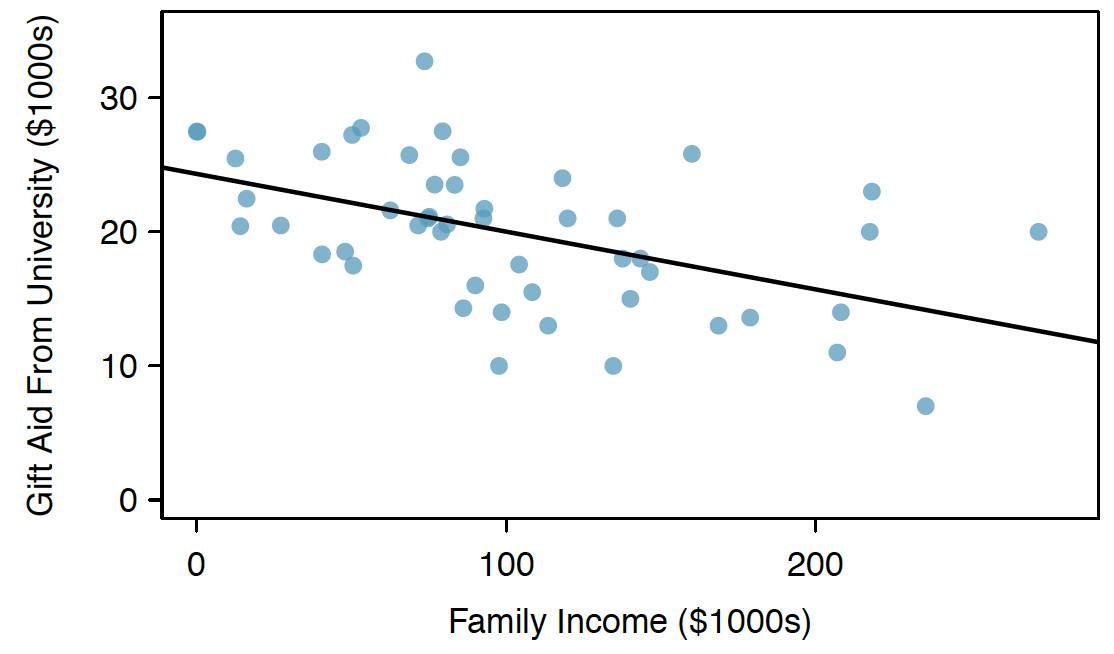
\includegraphics[width=0.8\textwidth]{figure/regression.png}
\end{center}

\end{frame}
%------------------------------------------------------------------------------


%------------------------------------------------------------------------------
\begin{frame}[fragile]
\frametitle{Questions for Today: Example From Text}
Using these values,
\begin{center}
\begin{tabular}{l|rr}
& family income & gift aid \\
& in \$1000's (x) & in \$1000's (y) \\ 
\hline
mean & $\overline{x}=101.8$ & $\overline{y}=19.94$ \\ 
sd & $s_x=63.2$ & $s_y=5.46$ \\ 
\hline
 &  & $R=-0.499$ \\ 
\hline
\end{tabular}
\end{center}

%
% Comment this
%
they fit the \blue{least-squares line}:
\pause
\begin{eqnarray*}
\widehat{y} &=& b_0 + b_1 x\\
\widehat{\mbox{aid}} &=& 24.3 - 0.0431 \times \mbox{family\_income}
\end{eqnarray*}
What do $24.3$ and $-0.0431$ mean?

\end{frame}
%------------------------------------------------------------------------------


%------------------------------------------------------------------------------
\begin{frame}[fragile]
\frametitle{Point Estimates of Intercept}
%
% Comment this
%
\blue{Point estimate of intercept $b_0$}: 24.3 (in \$1000's) describes the average aid if the family had no income.  

\vspace{0.25cm}
\pause
Here it is relevant since some families make no income, but the intercept may not make sense if there are no observations near $x=0$.  

\end{frame}
%------------------------------------------------------------------------------


%------------------------------------------------------------------------------
\begin{frame}[fragile]
\frametitle{Point Estimates of Slope}

%
% Comment this
%
\blue{Point estimate of slope $b_1$}: More interesting: it describes the \blue{relationship} between $x$ and $y$

\vspace{0.5cm}
\pause
In example: for each additional \$1000 of family income, we \blue{expect} a student to receive a difference of $\$1000 \times (-0.0431) = -\$43.10$ in aid on average.   

\vspace{0.5cm}
\pause
Even though we've labeled aid as the outcome variable, we are not positing a causal relationship; just an association.  


\end{frame}
%------------------------------------------------------------------------------


%------------------------------------------------------------------------------
\begin{frame}[fragile]
\frametitle{Extrapolate with Care}
\blue{Extrapolation}:  extend the application of a method or conclusion to an unknown situation by assuming that existing trends will continue or similar methods will be applicable.

%
% Comment this
%
\vspace{0.5cm}

\pause
What would be the gift aid given to a family with \$1,000,000 (i.e. $x=1000$) in family income?
\[
24.3 - 0.0431 \times 1000 = -18.8
\]
The school will take \$18,800 dollars away from you?  

\end{frame}
%------------------------------------------------------------------------------


%------------------------------------------------------------------------------
\begin{frame}[fragile]
\frametitle{Categorical Predictor $x$ With Two Levels}

%
% Comment this
%
$x$ can also be categorical.  

\vspace{0.25cm}
\pause
Ex: Ebay price for the video game Mario Kart. We convert the categorical $x$ into a \blue{indicator variable} $\mbox{cond\_new}$ which has 2 \blue{levels}:
\begin{enumerate}
\item $x=0$:  game is used. This is the \blue{baseline} level.
\item $x=1$:  game is new.
\end{enumerate}
\pause
The linear model is thus
\[
\widehat{\mbox{price}} = b_0 + b_1 \times \mbox{cond\_new}
\]

\end{frame}
%------------------------------------------------------------------------------


%------------------------------------------------------------------------------
\begin{frame}[fragile]
\frametitle{Categorical Predictor $x$ With Two Levels}

\begin{center}
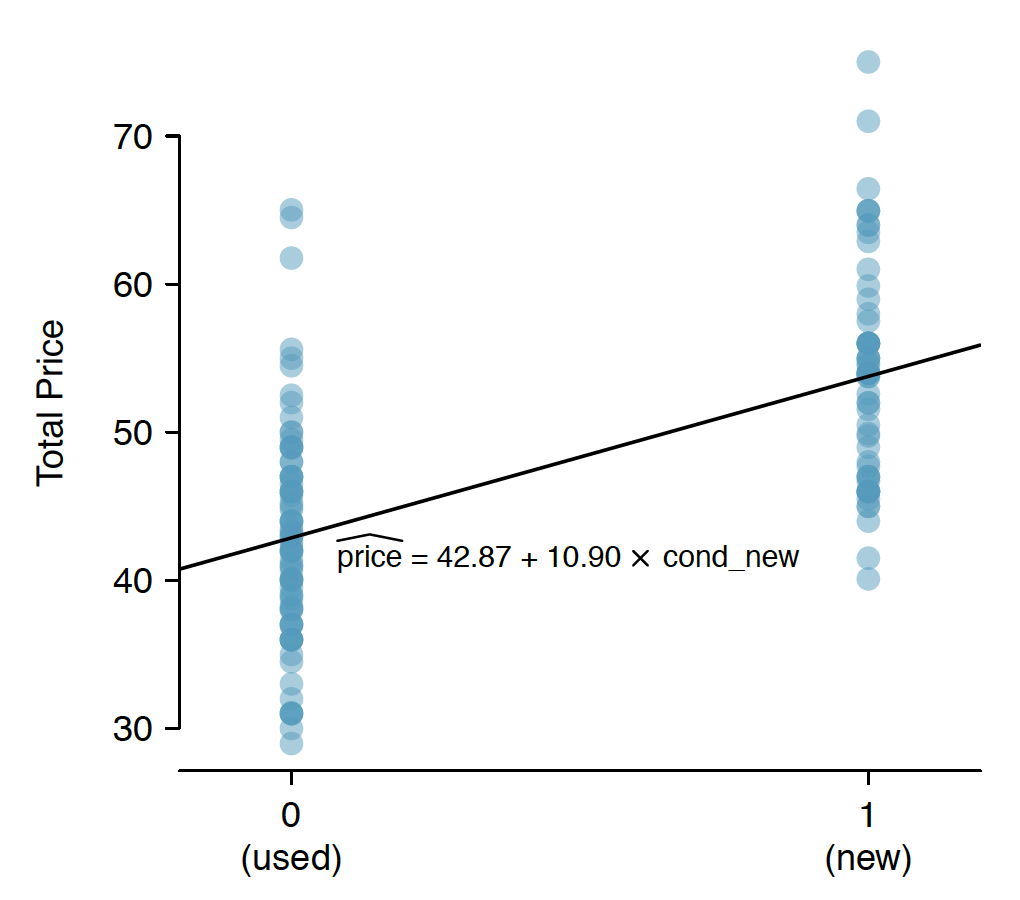
\includegraphics[width=0.8\textwidth]{figure/mario_kart.png}
\end{center}

\end{frame}
%------------------------------------------------------------------------------


%------------------------------------------------------------------------------
\begin{frame}[fragile]
\frametitle{Categorical Predictor $x$ With Two Levels}
%
% Comment this
%
The least-squares line is
\[
\widehat{\mbox{price}} = 42.87 + 10.90 \times \mbox{cond\_new}
\]
\pause
So when the game is
\begin{itemize}
\item Used, we have $x=0$, so the fitted value is $\$42.87 + \$0 = \$42.87$
\item New, we have $x=1$, so the fitted value is $\$42.87 + \$10.90 = \$53.77$
\end{itemize}
\pause
This can be generalized for predictor variables $x$ with more than two levels.

\end{frame}
%------------------------------------------------------------------------------


%------------------------------------------------------------------------------
\begin{frame}[fragile]
\frametitle{Types of Outliers in Linear Regression}
\begin{center}
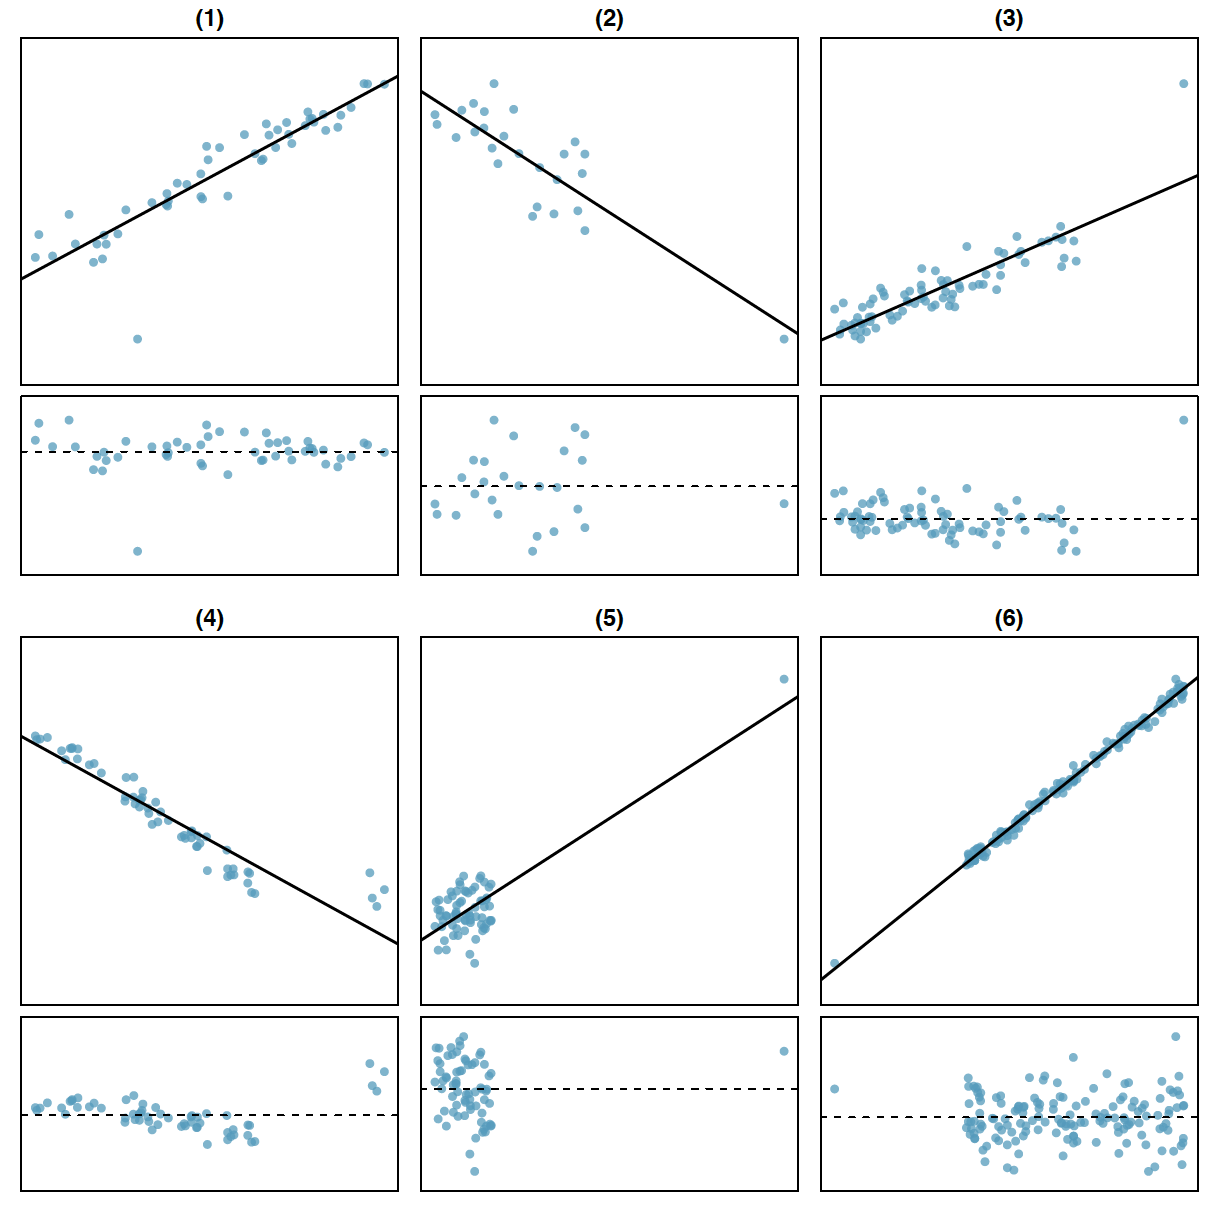
\includegraphics[height=0.8\textheight]{figure/outliers.png}
\end{center}
\end{frame}
%------------------------------------------------------------------------------


%------------------------------------------------------------------------------
\begin{frame}[fragile]
\frametitle{Types of Outliers in Linear Regression}
Especially in cases 3 and 5, the outliers seem to be pulling the least-squares line towards them.

\vspace{0.5cm}

\pause Points that fall horizontally away from the center of the cloud tend to pull harder on the line, so we call them points with high \blue{leverage}, i.e. large influence.  

\end{frame}
%------------------------------------------------------------------------------


%------------------------------------------------------------------------------
\begin{frame}[fragile]
\frametitle{Concept: Regression to the Mean}

The Madden Curse.  Many NFL players who feature on the cover of the video game Madden end up having subpar subsequent years, leading many to believe there is a curse.

\begin{center}

\includegraphics[height=0.7\textheight]{figure/MaddenCurse.jpg}
\end{center}


\end{frame}
%------------------------------------------------------------------------------


%------------------------------------------------------------------------------
\begin{frame}[fragile]
\frametitle{Concept: Regression to the Mean}

%
% Comment this.
%
\blue{Regression to the mean} is the phenomenon that if a variable is extreme on its first measurement, it will tend to be closer to the average on its second measurement.
\vspace{0.5cm}

\pause Madden is selecting players who had \blue{exceptional} seasons the previous year: the exceptional performance by the players who appear on the cover is \blue{not sustainable}.  

\vspace{0.5cm}

\pause So while it looks like a curse, it is just players reverting back to their ``mean'' level of performance.  

\end{frame}
%------------------------------------------------------------------------------


%%------------------------------------------------------------------------------
%\begin{frame}[fragile]
%\frametitle{Next Example}
%Are Higher Movie Budgets Associated with Higher IMDB Ratings for Movies Made from 1980-2005?  Guesses?
%
%\end{frame}
%%------------------------------------------------------------------------------


%%------------------------------------------------------------------------------
%\begin{frame}[fragile]
%\frametitle{Next Example}
%\pause But first, are the changes from
%\begin{itemize}
%\item 100 to 200
%\item 100,100 to 100,200
%\end{itemize}
%the same?

%We consider a $\log_{10}$ transformation:
%
%\begin{center}
%  \begin{tabular}{cc|c|cc}
%    $x$ & $y$ & $y-x$ & $\frac{y}{x}$ & $\log_{10}\left(\frac{y}{x}\right)$\\ 
%\hline
%    100 & 200 & 100 & 2 & 0.301\\ 
%    100100 & 100200 & 100 & 1.000999 & $0.00004342$\\ 
%    \pause 100000 & 200000 & 100000 & 2& \blue{0.301} \\ 
%  \end{tabular}
%\end{center}
%
%\pause Recall that $\log_{10}\left(\frac{y}{x}\right) = \log_{10}(y) - \log_{10}(x)$
%
%\vspace{0.5cm}
%
%\pause So we are considering \blue{multiplicative} changes, and not \blue{additive} changes.
%
%\end{frame}
%%------------------------------------------------------------------------------


%------------------------------------------------------------------------------
\begin{frame}[fragile]
\frametitle{Next Time}

Multiple Regression:  As opposed to \blue{simple linear regression} where there is only one predictor/explanatory variable $x$, we now consider \blue{many} predictors $x_1, x_2, \ldots$

\end{frame}
%------------------------------------------------------------------------------


\end{document}



%%------------------------------------------------------------------------------
%\begin{frame}[fragile]
%\frametitle{Midterm I Scores}
%Recall the analysis where we asked:  Did students who finished early do better?
%\begin{itemize}
%\item Explanatory variable $x$: submission rank
%\item Response variable $y$: midterm score
%\end{itemize}
%
%\begin{center}
%\includegraphics[width=0.7\textwidth]{midtermI.png}
%\end{center}
%
%\end{frame}
%%------------------------------------------------------------------------------
%
%
%%------------------------------------------------------------------------------
%\begin{frame}[fragile]
%\frametitle{Midterm I Scores}
%The output of the regression analysis:  
%\begin{table}[ht]
%\centering
%\begin{tabular}{r|rrrr}
%  \hline
% & Estimate & Std. Error & t value & Pr($>$$|$t$|$) \\ 
%  \hline
%(Intercept) & 20.5871 & 0.9460 & 21.76 & 0.0000 \\ 
%  submit rank & -0.0317 & 0.0516 & -0.61 & 0.5444 \\ 
%   \hline
%\end{tabular}
%\end{table}
%
%\vspace{0.25cm}
%\pause
%The point estimate $b_0 = 20.58$ of the intercept coefficient by itself doesn't mean anything: fitted score for someone who submitted at rank 0?
%
%\end{frame}
%%------------------------------------------------------------------------------
%
%
%%------------------------------------------------------------------------------
%\begin{frame}[fragile]
%\frametitle{Interpretation of Midterm I Scores Analysis Results}
%
%The point estimate $b_1=-0.0317$ of the slope coefficient means: for every increase in one in submission rank, we observe on average a \blue{decrease} of 0.0317 in the midterm I score.  
%
%\vspace{0.25cm}
%\pause
%Since $b_1$ is a point estimate based on $n=31$ $(x_i, y_i)$ pairs, we can associate a standard error (0.0516).  
%
%\vspace{0.25cm}
%\pause
%We conduct a two-sided hypothesis test of:
%\begin{eqnarray*}
%&& H_0: \beta_1 = 0\\
%\mbox{vs}&& H_A: \beta_1 \neq 0 
%\end{eqnarray*}
%thus the t-value is
%\[
%T = \frac{\mbox{point estimate}-\mbox{null value}}{\mbox{standard error}} = 
%\frac{-0.0317-0}{0.0516} = -0.61
%\]
%
%\vspace{0.25cm}
%\pause
%Pr($>$$|$t$|$) indicates the two-sided p-value of 0.5444. 
%
%\end{frame}
%%------------------------------------------------------------------------------
%
%
%%------------------------------------------------------------------------------
%\begin{frame}[fragile]
%\frametitle{Residuals Plot}
%\begin{center}
%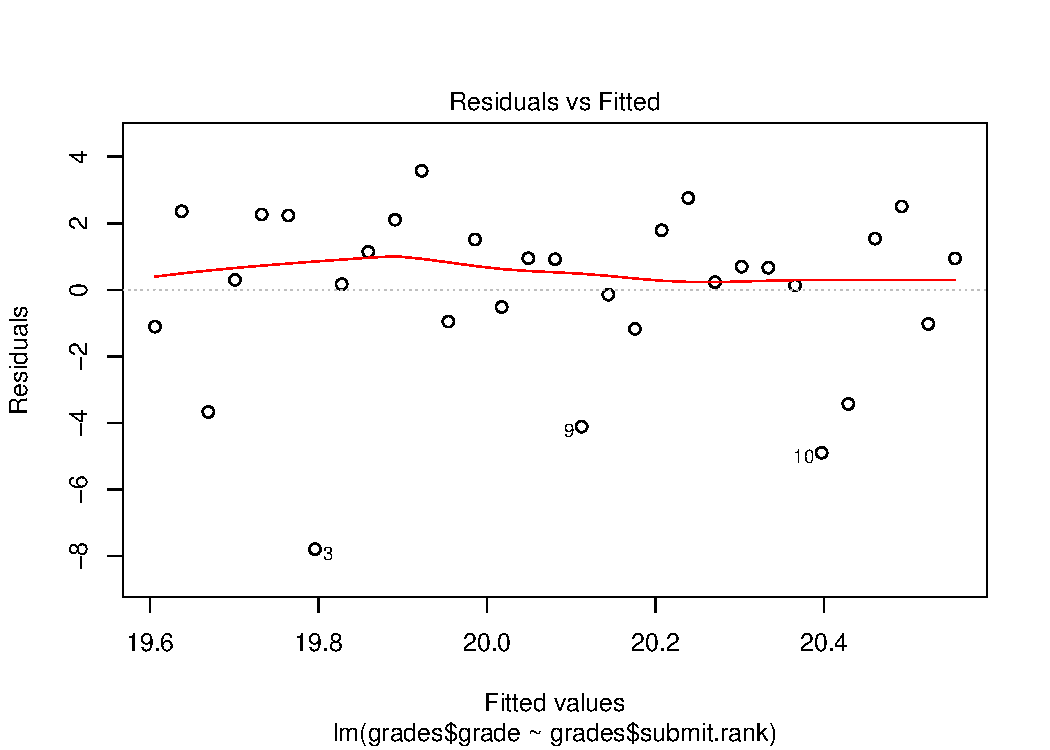
\includegraphics[width=\textwidth]{resid1.pdf}
%\end{center}
%\end{frame}
%%------------------------------------------------------------------------------
%
%
%%------------------------------------------------------------------------------
%\begin{frame}[fragile]
%\frametitle{QQ-Plot of (Standardized) Residuals}
%\begin{center}
%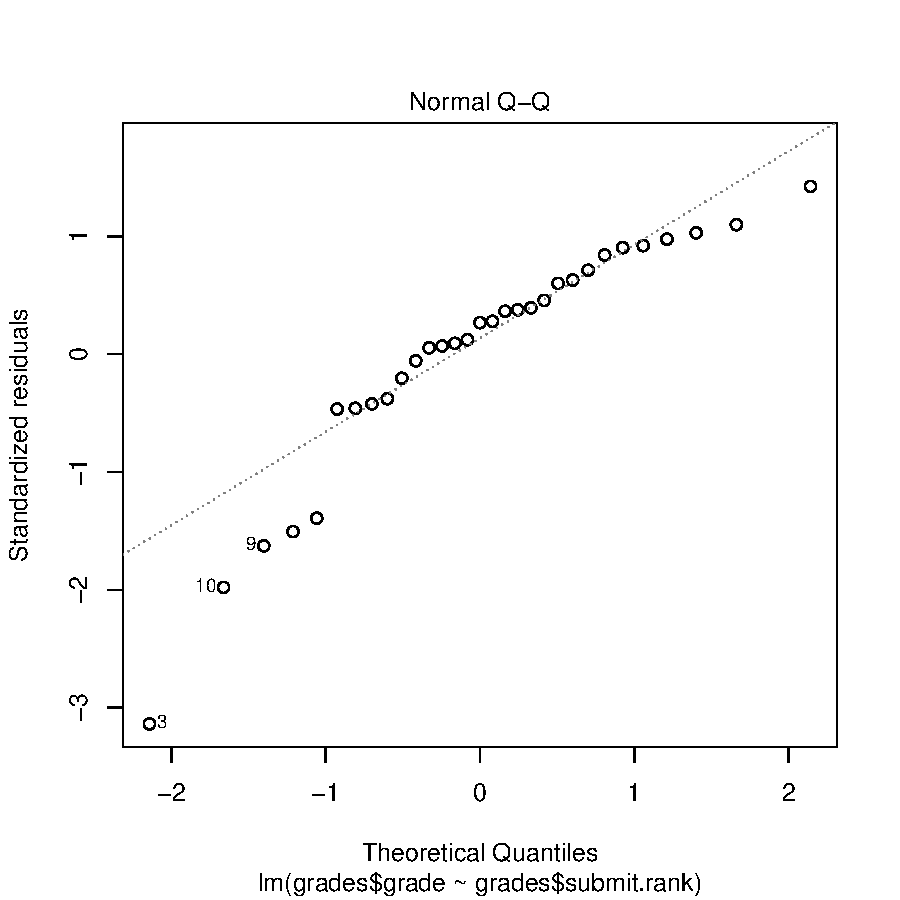
\includegraphics[width=0.7\textwidth]{resid2.pdf}
%\end{center}
%\end{frame}
%%------------------------------------------------------------------------------
